\begin{figure}[t]
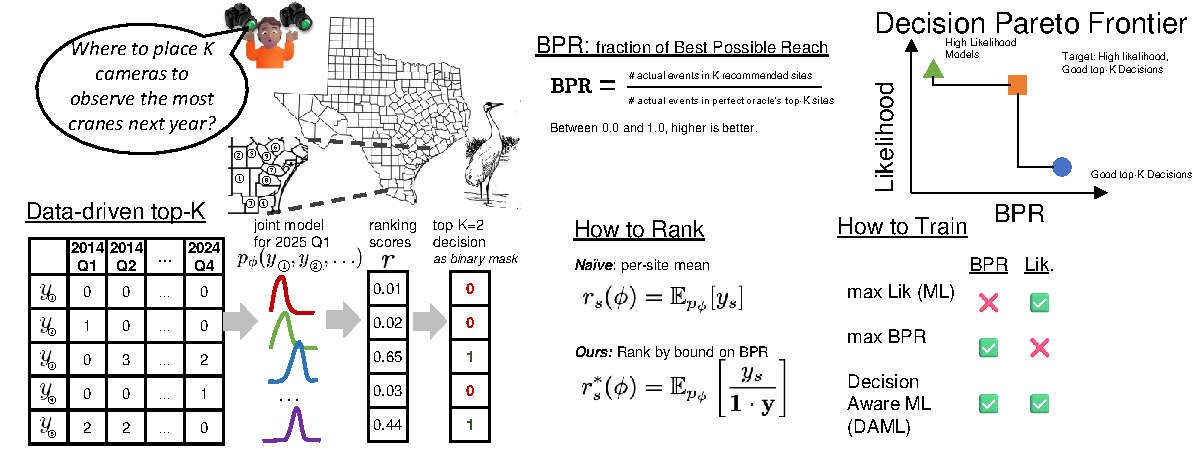
\includegraphics[width=1\textwidth]{figures/overview_figure.pdf}
\caption[Visual overview of our approach and contributions to the \emph{how to rank} and \emph{how to train} open problems.]{
Visual overview of our approach and contributions to the \emph{how to rank} and \emph{how to train} open problems.
%\textbf{Decision making with limited resources}. (left) Pictured is a cartoon dataset representing sightings of an endangered bird in the counties of a state. Imagine, before this data is observed, the state conservation department wishes to allocate resources to the counties with top-4 highest amounts of bird sightings. (center) This cartoon represents the predictions made by a model trained to maximize likelihood. This model has correctly allocated most of the probability mass to the cluster of bird sightings in the center of the states. However, this model has missed the top-4 counties entirely. (right) This cartoon represents the predictions made by a model trained to optimize the proportion of correct predictions in the top-4. While the likelihood of this model would be low: it places almost no probability in the middle of the state, it correctly recovers the top-4 counties.
}%end caption
\label{fig:cartoon_exp}
\end{figure}
